%!TEX TS-program = pdflatex
%!TEX root = example02.tex

\section{Main Part}

\lipsum[11-13]

% an equation
\begin{equation}
    \Mmat = \Rmat
\end{equation}

% a simple figure
\begin{figure}[t]
    \centering
    \includestandalone{./images/matrix}
    \caption{A simple figures including the use of macros to typeset a matrix \Mmat.}
    \label{fig:matrix}
\end{figure}

\lipsum[14-15]

% subfigures using the subcaption package
\begin{figure}[t]
    \centering
    \begin{subfigure}[b]{0.49\textwidth}
        \centering
        \begin{tikzpicture}
    \draw(1,1) rectangle (5,5);
\end{tikzpicture}

        \caption{A simple square.}
        \label{fig:squareSimple}
    \end{subfigure}
    \begin{subfigure}[b]{0.49\textwidth}
        \centering
        \includestandalone{./figs/squareFilled}
        \caption{A filled square.}
        \label{fig:squareFilled}
    \end{subfigure}
    \caption{Using the \emph{subcaption} package to draw a simple and a filled square.}
    \label{fig:squares}
\end{figure}

\lipsum[16-17]

% a simple table
\begin{table}[t]
    \centering
    \begin{tabular}{ccc}\toprule
        Column 1 & Column 2 & Column 3\\\bottomrule\toprule
        Entry 1  & Entry 2  & Entry 3 \\\bottomrule
    \end{tabular}
    \caption{A simple table.}
    \label{tab:table}
\end{table}

\lipsum[17-18]

% subfigures using pgfplots and the subcaption package
\begin{figure}
    \centering
    \begin{subfigure}[b]{0.49\textwidth}
        \begin{tikzpicture}
            \begin{axis}[width=\columnwidth,xlabel=$x$,ylabel=$y$]
                \addplot{x};
            \end{axis}
        \end{tikzpicture}
    \end{subfigure}
    \begin{subfigure}[b]{0.49\textwidth}
        \begin{tikzpicture}
            \begin{axis}[width=\columnwidth,xlabel=$x$,ylabel=$y$]
                \addplot{x^2};
            \end{axis}
        \end{tikzpicture}
    \end{subfigure}
    \caption{Using the \emph{subcaption} package to draw simple pgfplot environments plotting $y=x$ and $y=x^2$.}
    \label{fig:pgfplot}
\end{figure}

\lipsum[18-19]

% an algorithm
\begin{algorithm}[t]
 \SetAlgoLined
  \KwData{Data for the algorithm}
  \KwResult{Result of the algorithm}
  \Repeat{finished}{
      Compute something. \\
  }
  \caption{An algorithm.} 
  \label{algo:algorithm}
\end{algorithm}

\lipsum[20-21]

% a remark
\begin{remark}
    A brief remark.
\end{remark}

\lipsum[22-23]

% a simple comment block
\begin{comment}
    A comment block.
\end{comment}

\lipsum[24-25]

% a figure in a comment block and outside of a comment block
\begin{comment}
\begin{figure}[t]
    \centering
    \includestandalone{./images/matrix}
    \caption{A matrix $\mathbf{M}$.}
    \label{fig:matrix1}
\end{figure}
\end{comment}
\begin{figure}[t]
    \centering
    \includestandalone{./images/matrix}
    \caption{This figure is only shown once since \emph{comment} environments are not printed.}
    \label{fig:matrix2}
\end{figure}

\lipsum[26-27]

% avoiding multiple tikzpicture environments in one figure
\begin{figure}
    \centering
    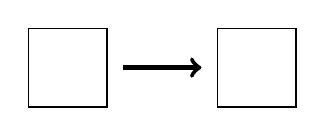
\begin{tikzpicture}
        \begin{scope}
            \draw (0,0) rectangle (1,1);
        \end{scope}
        \begin{scope}[xshift=1.2cm]
            \draw[->,ultra thick] (0,0.5) -- (1,0.5);
        \end{scope}
        \begin{scope}[xshift=2.4cm]
            \draw (0,0) rectangle (1,1);
        \end{scope}
    \end{tikzpicture}
    \caption{Multiple scopes in one \emph{tikzpicture} environment.}
    \label{fig:scopes}
\end{figure}
